David Rohrbaugh

2014-11-14

The Samantha Module, and Electronics

\begin{tabular}{|p{5cm}|p{5cm}|}
 \hline
 This week, I worked on the electronics with Nick. We finished implementing power poles into our wiring, and put the wiring back on the robot, but better this time. The Samantha Module seems to not be working, but a real test will have to be run.
 &
 The configuration of the electronics was changed, so the power poles are a little bit out of wack. This can be fixed, however.
 \\
 \hline
\end{tabular}

\medskip

This is a diagram of our current wiring, but separate from the robot to aid comprehension.

\begin{center}
 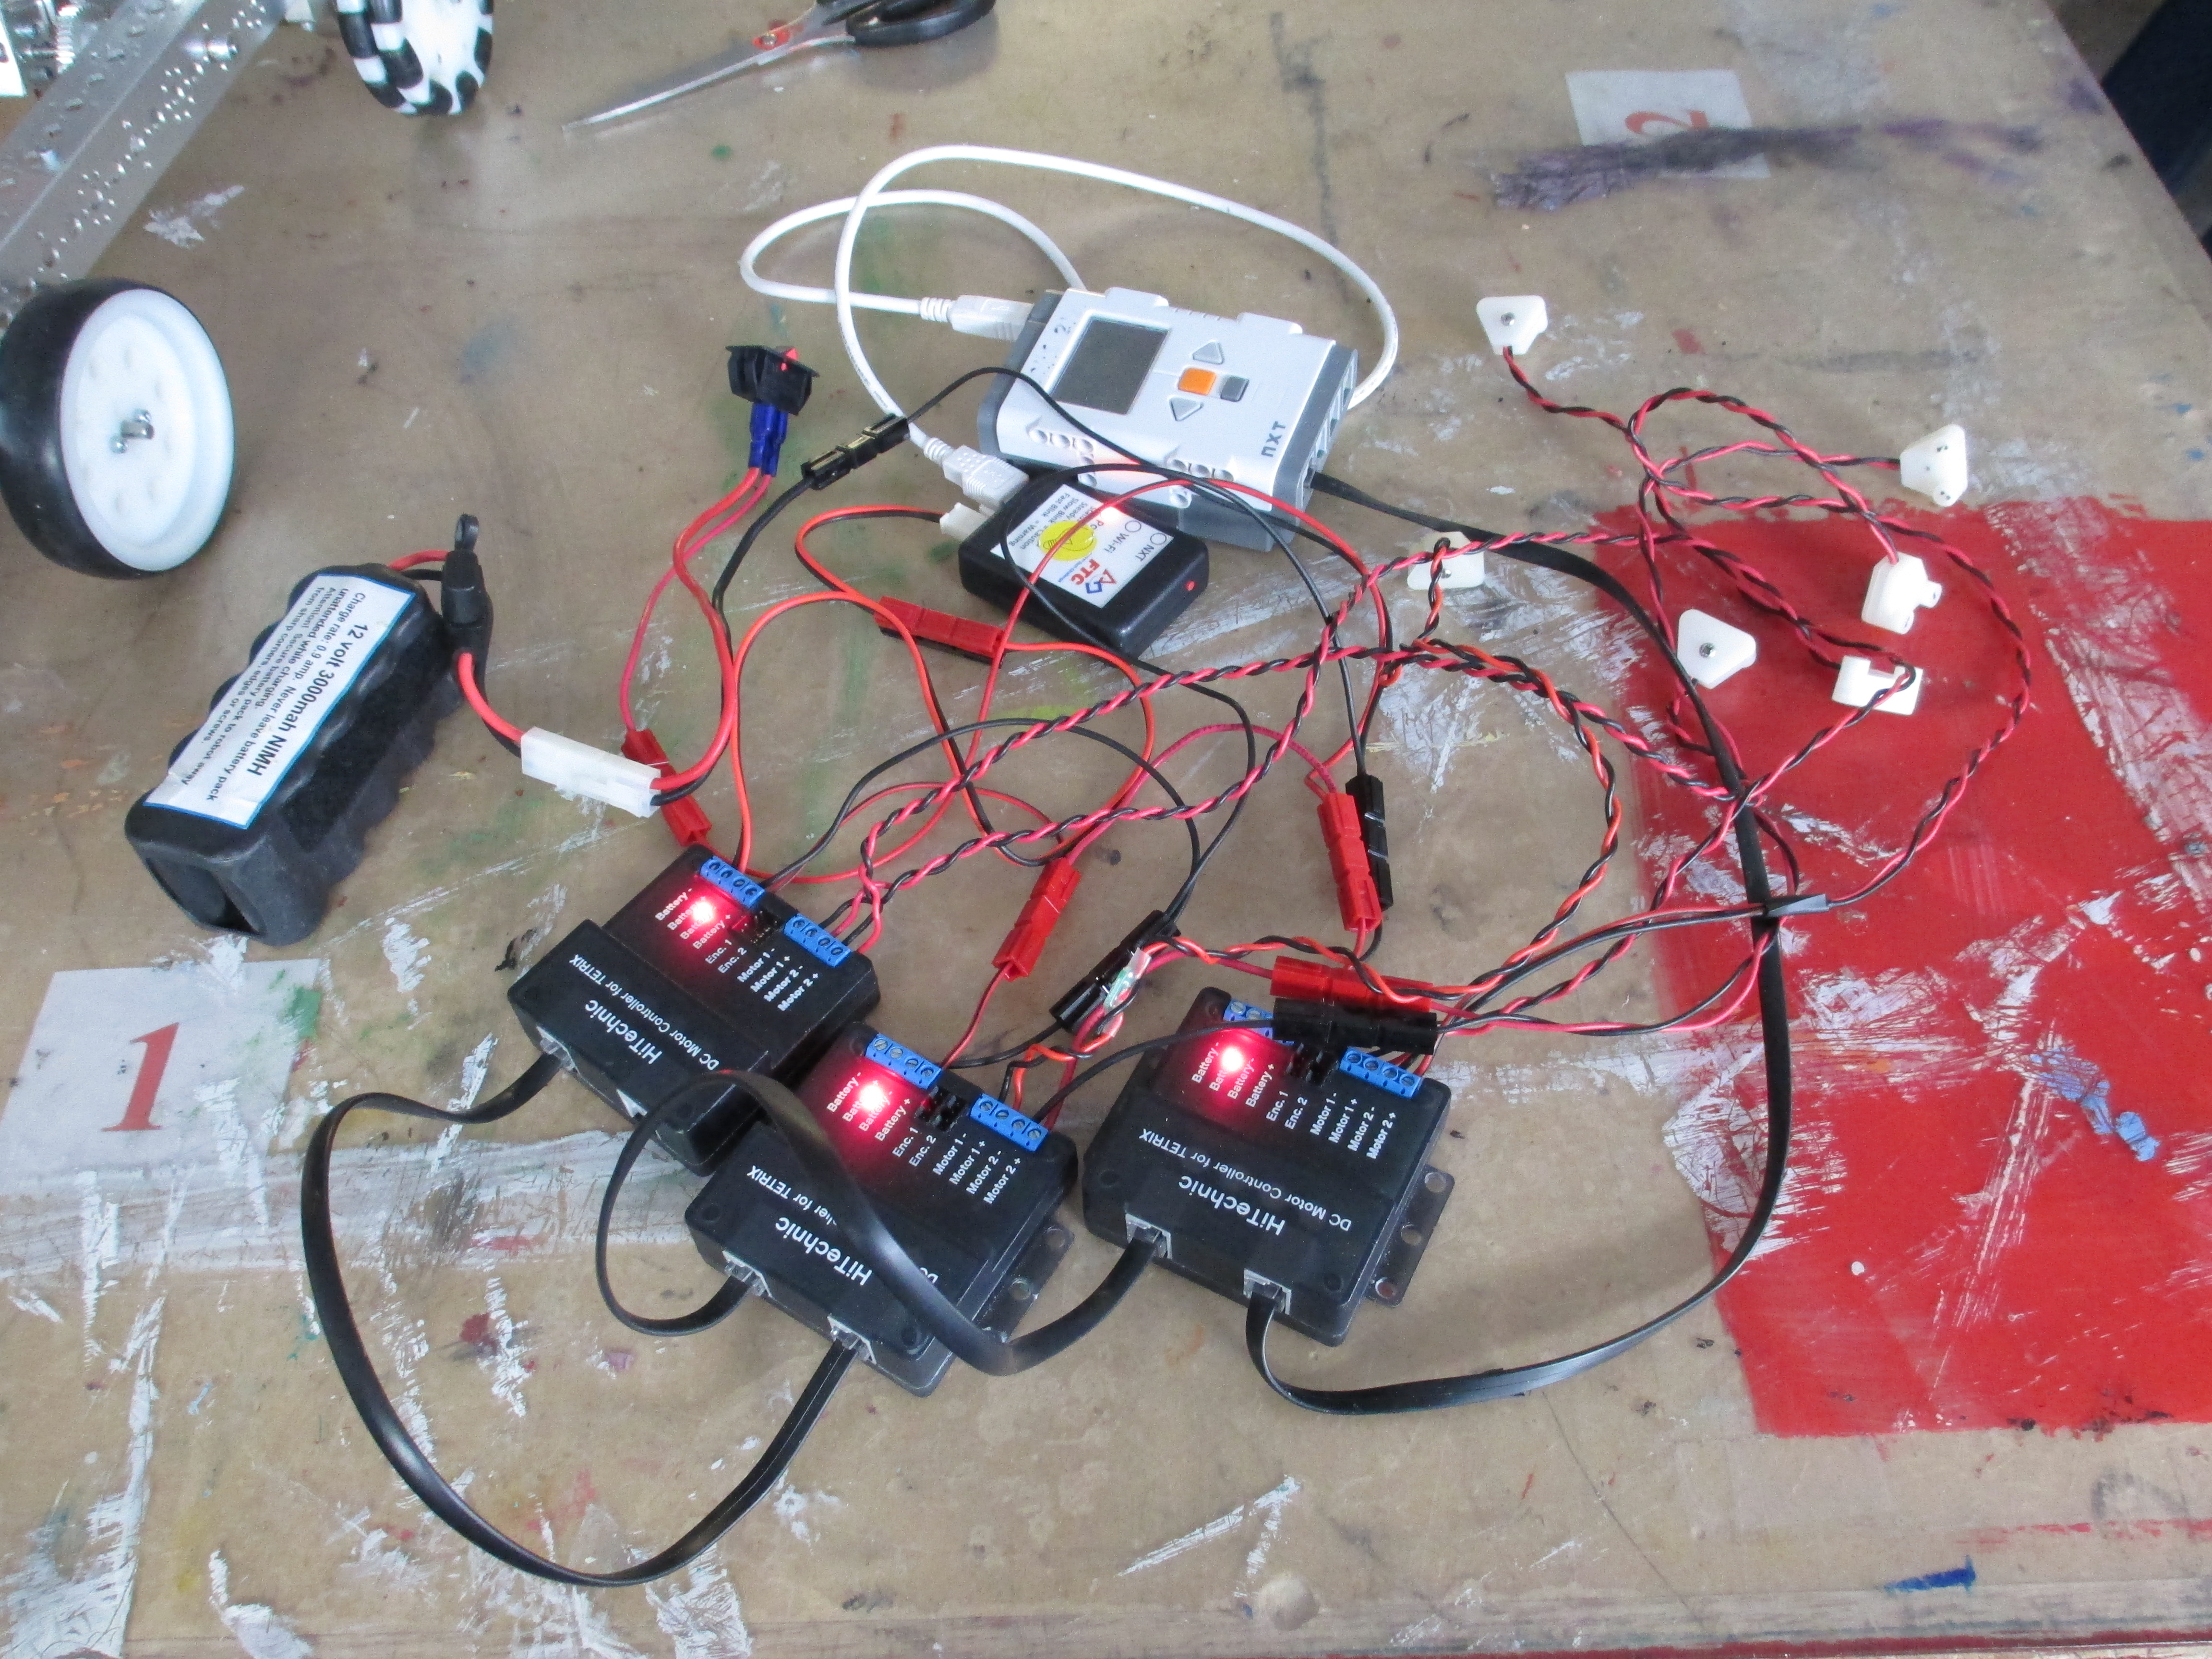
\includegraphics[width=\textwidth]{./Entries/Images/detached_wiring.jpg}
\end{center}
